\section{Class Description}
\subsection{Example}
\subsubsection{App}
\begin{wrapfigure}{l}{4.5cm}
    \raisebox{0pt}[\dimexpr\height-0.5\baselineskip\relax]{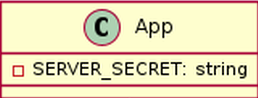
\includegraphics[width=4.5cm]{classes/auth/app.png}}
\end{wrapfigure} 
\par
The main class of the authentication service.
\newline
\newline
\textbf{Attributes}
\begin{itemize}
    \item \textbf{SERVER\_SECRET} the encryption key that is shared among all the services to decrypt tokens
\end{itemize}

\subsection{Authentication}

\subsubsection{User Model}
\begin{wrapfigure}{l}{4.5cm}
    \raisebox{0pt}[\dimexpr\height-0.5\baselineskip\relax]{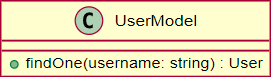
\includegraphics[width=4.5cm]{classes/auth/1.png}}
\end{wrapfigure} 
\par
The collection of registered users in the database.
\newline
\newline
\textbf{Methods}
\begin{itemize}
    \item \textbf{findOne} returns the user that has the matching username
\end{itemize}

\subsubsection{User}
\begin{wrapfigure}{l}{4.5cm}
    \raisebox{0pt}[\dimexpr\height-0.5\baselineskip\relax]{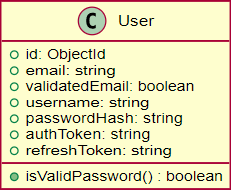
\includegraphics[width=4.5cm]{classes/auth/2.png}}
\end{wrapfigure} 
\par
A registered user
\newline
\newline
\textbf{Attributes}
\begin{itemize}
    \item \textbf{email} email of the user
    \item \textbf{validatedEmail} iff the email is validated
    \item \textbf{username} username of the user
    \item \textbf{passwordHash} hash of the password of the user
    \item \textbf{authToken} the current authentication token of the user
    \item \textbf{refreshToken} the current refresh token of the user
\end{itemize}
\textbf{Methods}
\begin{itemize}
    \item \textbf{isValidPassword} iff the supplied password is valid
\end{itemize}

\subsubsection{EmailValidator}
\begin{wrapfigure}{l}{4.5cm}
    \raisebox{0pt}[\dimexpr\height-0.5\baselineskip\relax]{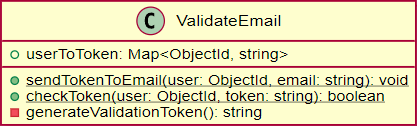
\includegraphics[width=4.5cm]{classes/auth/3.png}}
\end{wrapfigure} 
\par
This static class sends an email to the user with a token and checks if the given token is correct.
\newline
\newline
\textbf{Attributes}
\begin{itemize}
    \item \textbf{userToToken} maps the user id to the sent token
\end{itemize}
\textbf{Methods}
\begin{itemize}
    \item \textbf{sendTokenToEmail} sends a token to the given email 
    \item \textbf{checkToken} compares the received token with the token sent to email
    \item \textbf{generateValidationToken} generates a validation token
\end{itemize}

\subsubsection{TokenContent}
\begin{wrapfigure}{l}{4.5cm}
    \raisebox{0pt}[\dimexpr\height-0.5\baselineskip\relax]{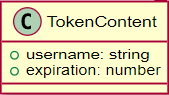
\includegraphics[width=4.5cm]{classes/auth/4.png}}
\end{wrapfigure} 
\par
This class depicts a unencrypted access token.
\newline
\newline
\textbf{Attributes}
\begin{itemize}
    \item \textbf{username} username of the owner of the token
    \item \textbf{expiration} expiration time of the token
\end{itemize}

\subsection{Workspace Management}

\subsubsection{WorkspaceModel}
\begin{wrapfigure}{l}{4.5cm}
    \raisebox{0pt}[\dimexpr\height-0.5\baselineskip\relax]{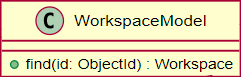
\includegraphics[width=4.5cm]{classes/workspace-management/1.png}}
\end{wrapfigure} 
\par
The collection of workspaces in the database.
\newline
\newline
\textbf{Methods}
\begin{itemize}
    \item \textbf{find} returns the workspace with the given ID.
\end{itemize}

\subsubsection{Workspace}
\begin{wrapfigure}{l}{4.5cm}
    \raisebox{0pt}[\dimexpr\height-0.5\baselineskip\relax]{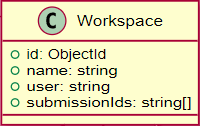
\includegraphics[width=4.5cm]{classes/workspace-management/2.png}}
\end{wrapfigure} 
\par
The document that includes all the relevant information about a workspace.
\newline
\newline
\textbf{Attributes}
\begin{itemize}
    \item \textbf{name} name of the workspace
    \item \textbf{user} user of the workspace
    \item \textbf{submissionIds} all valid submission IDs of the workspace
\end{itemize}

\subsubsection{SensorType}
\begin{wrapfigure}{l}{4.5cm}
    \raisebox{0pt}[\dimexpr\height-0.5\baselineskip\relax]{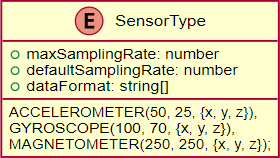
\includegraphics[width=4.5cm]{classes/workspace-management/4.png}}
\end{wrapfigure} 
\par
This enumeration consists of the supported sensors.
\newline
\newline
\textbf{Attributes}
\begin{itemize}
    \item \textbf{maxSamplingRate} the maximum sampling rate of the sensor
    \item \textbf{defaultSamplingRate} the default sampling rate of the sensor
    \item \textbf{dataFormat} the data format of the sensor
\end{itemize}

\subsubsection{Sensor}
\begin{wrapfigure}{l}{4.5cm}
    \raisebox{0pt}[\dimexpr\height-0.5\baselineskip\relax]{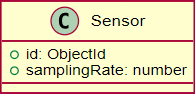
\includegraphics[width=4.5cm]{classes/workspace-management/3.png}}
\end{wrapfigure} 
\par
This class represents a chosen sensor of the workspace. 
\newline
\newline

\textbf{Attributes}
\begin{itemize}
    \item \textbf{samplingRate} the selected sampling rate of the sensor
\end{itemize}

\subsubsection{Label}
\begin{wrapfigure}{l}{4.5cm}
    \raisebox{0pt}[\dimexpr\height-0.5\baselineskip\relax]{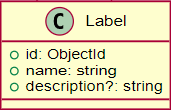
\includegraphics[width=4.5cm]{classes/workspace-management/5.png}}
\end{wrapfigure} 
\par
This class represent an action that describes a sample.
\newline
\newline
\textbf{Attributes}
\begin{itemize}
    \item \textbf{name} name of the label
    \item \textbf{description} description of the label
\end{itemize}

\subsubsection{SampleModel}
\begin{wrapfigure}{l}{4.5cm}
    \raisebox{0pt}[\dimexpr\height-0.5\baselineskip\relax]{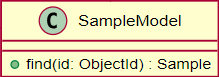
\includegraphics[width=4.5cm]{classes/workspace-management/6.png}}
\end{wrapfigure} 
\par
The collection of samples in the database.
\newline
\newline
\textbf{Methods}
\begin{itemize}
    \item \textbf{find} returns the sample with the given ID.
\end{itemize}

\subsubsection{Sample}
\begin{wrapfigure}{l}{4.5cm}
    \raisebox{0pt}[\dimexpr\height-0.5\baselineskip\relax]{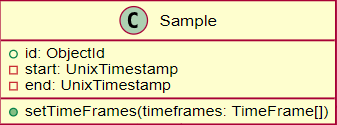
\includegraphics[width=4.5cm]{classes/workspace-management/7.png}}
\end{wrapfigure} 
\par
This class represents a document in the database that contains raw sensor data, its selected timeframes and its label.
\newline
\newline
\textbf{Attributes}
\begin{itemize}
    \item \textbf{start} the timestamp of the start of recording
    \item \textbf{end} the timestamp of the end of recording
\end{itemize}
\textbf{Methods}
\begin{itemize}
    \item \textbf{setTimeFrames} sets the timeframes of the sample
\end{itemize}

\subsubsection{SensorDataPoints}
\begin{wrapfigure}{l}{4.5cm}
    \raisebox{0pt}[\dimexpr\height-0.5\baselineskip\relax]{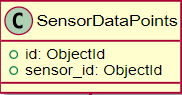
\includegraphics[width=4.5cm]{classes/workspace-management/8.png}}
\end{wrapfigure} 
\par
This class represents data points of a specific sensor.
\newline
\newline
\textbf{Attributes}
\begin{itemize}
    \item \textbf{sensor\_id} the ID of the sensor to which the data belongs
\end{itemize}

\subsubsection{DataPoint}
\begin{wrapfigure}{l}{4.5cm}
    \raisebox{0pt}[\dimexpr\height-0.5\baselineskip\relax]{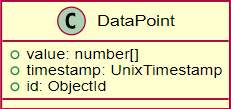
\includegraphics[width=4.5cm]{classes/workspace-management/9.png}}
\end{wrapfigure} 
\par
This class is blablabla and bla bla bla. This denotes bla bla bla and provided by Selehaddin Ozdemir. xdaslkads anu adl kl;asd k;lads l;l;kasdk ;lkdsa;k lllld kksdk mjdask hdaksjhd haso sadjh salk da.
\newline
\newline
\textbf{Attributes}
\begin{itemize}
    \item \textbf{value}
    \item \textbf{timestamp}
\end{itemize}

\subsubsection{TimeFrame}
\begin{wrapfigure}{l}{4.5cm}
    \raisebox{0pt}[\dimexpr\height-0.5\baselineskip\relax]{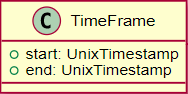
\includegraphics[width=4.5cm]{classes/workspace-management/10.png}}
\end{wrapfigure} 
\par
This class is blablabla and bla bla bla. This denotes bla bla bla and provided by Selehaddin Ozdemir. xdaslkads anu adl kl;asd k;lads l;l;kasdk ;lkdsa;k lllld kksdk mjdask hdaksjhd haso sadjh salk da.
\newline
\newline
\textbf{Attributes}
\begin{itemize}
    \item \textbf{start}
    \item \textbf{end}
\end{itemize}

\subsection{Model Management}

\subsubsection{Trainer}
\begin{wrapfigure}{l}{4.5cm}
    \raisebox{0pt}[\dimexpr\height-0.5\baselineskip\relax]{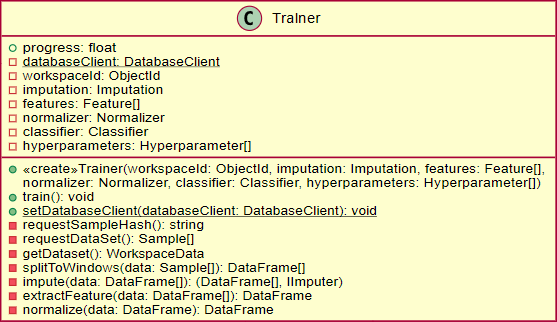
\includegraphics[width=4.5cm]{classes/model-management/1.png}}
\end{wrapfigure} 
\par
This class is blablabla and bla bla bla. This denotes bla bla bla and provided by Selehaddin Ozdemir. xdaslkads anu adl kl;asd k;lads l;l;kasdk ;lkdsa;k lllld kksdk mjdask hdaksjhd haso sadjh salk da.
\newline
\newline
\textbf{Attributes}
\begin{itemize}
    \item \textbf{progress}
    \item \textbf{databaseClient}
    \item \textbf{workspaceId}
    \item \textbf{imputation}
    \item \textbf{features}
    \item \textbf{normalizer}
    \item \textbf{classifier}
    \item \textbf{hyperparameters}
\end{itemize}
\textbf{Methods}
\begin{itemize}
    \item \textbf{train}
    \item \textbf{setDatabaseClient}
    \item \textbf{requestSampleHash}
    \item \textbf{requestDataSet}
    \item \textbf{splitToWindows}
    \item \textbf{impute}
    \item \textbf{extractFeature}
    \item \textbf{normalize}
\end{itemize}

\subsubsection{Workspace}
\begin{wrapfigure}{l}{4.5cm}
    \raisebox{0pt}[\dimexpr\height-0.5\baselineskip\relax]{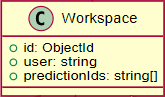
\includegraphics[width=4.5cm]{classes/model-management/2.png}}
\end{wrapfigure} 
\par
This class is blablabla and bla bla bla. This denotes bla bla bla and provided by Selehaddin Ozdemir. xdaslkads anu adl kl;asd k;lads l;l;kasdk ;lkdsa;k lllld kksdk mjdask hdaksjhd haso sadjh salk da.
\newline
\newline
\textbf{Attributes}
\begin{itemize}
    \item \textbf{user}
    \item \textbf{predictionIds}
\end{itemize}

\subsubsection{Sensor}
\begin{wrapfigure}{l}{4.5cm}
    \raisebox{0pt}[\dimexpr\height-0.5\baselineskip\relax]{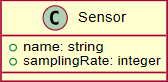
\includegraphics[width=4.5cm]{classes/model-management/3.png}}
\end{wrapfigure} 
\par
This class is blablabla and bla bla bla. This denotes bla bla bla and provided by Selehaddin Ozdemir. xdaslkads anu adl kl;asd k;lads l;l;kasdk ;lkdsa;k lllld kksdk mjdask hdaksjhd haso sadjh salk da.
\newline
\newline
\textbf{Attributes}
\begin{itemize}
    \item textbf{name}
    \item textbf{samplingRate}
\end{itemize}

\subsubsection{MLModel}
\begin{wrapfigure}{l}{4.5cm}
    \raisebox{0pt}[\dimexpr\height-0.5\baselineskip\relax]{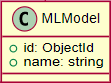
\includegraphics[width=4.5cm]{classes/model-management/4.png}}
\end{wrapfigure} 
\par
This class is blablabla and bla bla bla. This denotes bla bla bla and provided by Selehaddin Ozdemir. xdaslkads anu adl kl;asd k;lads l;l;kasdk ;lkdsa;k lllld kksdk mjdask hdaksjhd haso sadjh salk da.
\newline
\newline
\textbf{Attributes}
\begin{itemize}
    \item \textbf{name}
\end{itemize}

\subsubsection{Imputation}
\begin{wrapfigure}{l}{4.5cm}
    \raisebox{0pt}[\dimexpr\height-0.5\baselineskip\relax]{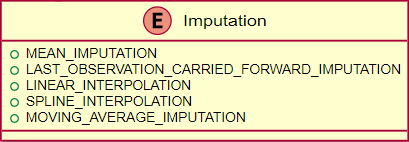
\includegraphics[width=4.5cm]{classes/model-management/5.png}}
\end{wrapfigure} 
\par
This class is blablabla and bla bla bla. This denotes bla bla bla and provided by Selehaddin Ozdemir. xdaslkads anu adl kl;asd k;lads l;l;kasdk ;lkdsa;k lllld kksdk mjdask hdaksjhd haso sadjh salk da.
\newline
\newline

\subsubsection{Feature}
\begin{wrapfigure}{l}{4.5cm}
    \raisebox{0pt}[\dimexpr\height-0.5\baselineskip\relax]{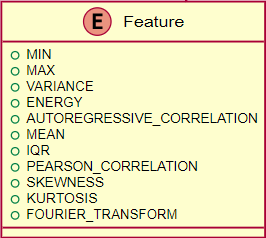
\includegraphics[width=4.5cm]{classes/model-management/6.png}}
\end{wrapfigure} 
\par
This class is blablabla and bla bla bla. This denotes bla bla bla and provided by Selehaddin Ozdemir. xdaslkads anu adl kl;asd k;lads l;l;kasdk ;lkdsa;k lllld kksdk mjdask hdaksjhd haso sadjh salk da.
\newline
\newline
\newline
\newline

\subsubsection{Normalizer}
\begin{wrapfigure}{l}{4.5cm}
    \raisebox{0pt}[\dimexpr\height-0.5\baselineskip\relax]{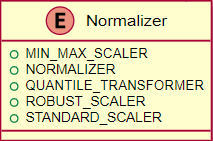
\includegraphics[width=4.5cm]{classes/model-management/7.png}}
\end{wrapfigure} 
\par
This class is blablabla and bla bla bla. This denotes bla bla bla and provided by Selehaddin Ozdemir. xdaslkads anu adl kl;asd k;lads l;l;kasdk ;lkdsa;k lllld kksdk mjdask hdaksjhd haso sadjh salk da.
\newline
\newline

\subsubsection{Factory}
\begin{wrapfigure}{l}{4.5cm}
    \raisebox{0pt}[\dimexpr\height-0.5\baselineskip\relax]{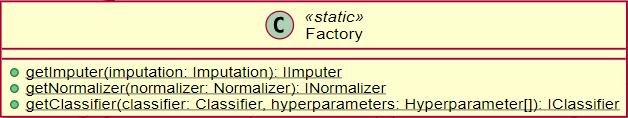
\includegraphics[width=4.5cm]{classes/model-management/8.png}}
\end{wrapfigure} 
\par
This static class is responsible for creating imputer, normalizer and classifier objects.
\newline
\newline
\textbf{Methods}
\begin{itemize}
    \item \textbf{getImputer} creates and returns an imputer object with the given name of the imputer
    \item \textbf{getNormalizer} creates and returns a normalizer object with the given name of the normalizer
    \item \textbf{getClassifier} creates and returns a classifier object with the given name of the classifier
\end{itemize}

\subsubsection{IImputer}
\begin{wrapfigure}{l}{4.5cm}
    \raisebox{0pt}[\dimexpr\height-0.5\baselineskip\relax]{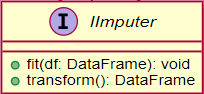
\includegraphics[width=4.5cm]{classes/model-management/9.png}}
\end{wrapfigure} 
\par
This is an interface for an imputer object.
\newline
\newline
\textbf{Methods}
\begin{itemize}
    \item \textbf{fit} fits the given data in the imputer object
    \item \textbf{transform} imputes the given data
\end{itemize}

\subsubsection{INormalizer}
\begin{wrapfigure}{l}{4.5cm}
    \raisebox{0pt}[\dimexpr\height-0.5\baselineskip\relax]{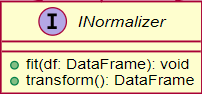
\includegraphics[width=4.5cm]{classes/model-management/10.png}}
\end{wrapfigure} 
\par
This is an interface for a normalizer object.
\newline
\newline
\textbf{Methods}
\begin{itemize}
    \item \textbf{fit} fits the given data in the normalizer object
    \item \textbf{transform} normalizes the given data
\end{itemize}

\subsubsection{IClassifier}
\begin{wrapfigure}{l}{4.5cm}
    \raisebox{0pt}[\dimexpr\height-0.5\baselineskip\relax]{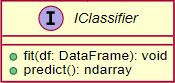
\includegraphics[width=4.5cm]{classes/model-management/11.png}}
\end{wrapfigure} 
\par
This is an interface for a classifier object.
\newline
\newline
\textbf{Methods}
\begin{itemize}
    \item \textbf{fit} fits the given data in the classifier object
    \item \textbf{predict} predicts of which label this data is
\end{itemize}

\subsubsection{PerfomanceMetrics}
\begin{wrapfigure}{l}{4.5cm}
    \raisebox{0pt}[\dimexpr\height-0.5\baselineskip\relax]{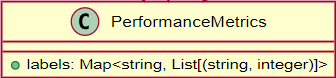
\includegraphics[width=4.5cm]{classes/model-management/12.png}}
\end{wrapfigure} 
\par
This class represents the performance metrics of a trained model.
\newline
\newline
\textbf{Attributes}
\begin{itemize}
    \item \textbf{labels} map of labels to their performance metrics
\end{itemize}

\subsubsection{Hyperparameter}
\begin{wrapfigure}{l}{4.5cm}
    \raisebox{0pt}[\dimexpr\height-0.5\baselineskip\relax]{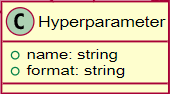
\includegraphics[width=4.5cm]{classes/model-management/13.png}}
\end{wrapfigure} 
\par
This class represents a hyperparameter for training a model.
\newline
\newline
\textbf{Attributes}
\begin{itemize}
    \item \textbf{name} name of the hyperparameter
    \item \textbf{format} the format of the value that the hyperparameter can get
\end{itemize}

\subsubsection{WorkspaceData}
\begin{wrapfigure}{l}{4.5cm}
    \raisebox{0pt}[\dimexpr\height-0.5\baselineskip\relax]{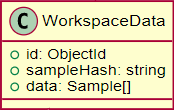
\includegraphics[width=4.5cm]{classes/model-management/14.png}}
\end{wrapfigure} 
\par
This class holds the sample data from the last training.
\newline
\newline
\textbf{Attributes}
\begin{itemize}
    \item \textbf{sampleHash} hash of the sample data
    \item \textbf{data} the sample data
\end{itemize}

\subsubsection{SlidingWindow}
\begin{wrapfigure}{l}{4.5cm}
    \raisebox{0pt}[\dimexpr\height-0.5\baselineskip\relax]{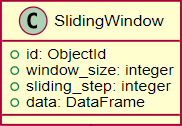
\includegraphics[width=4.5cm]{classes/model-management/15.png}}
\end{wrapfigure} 
\par
This class hold the sample data from recent trainings which is split into windows.
\newline
\newline
\textbf{Attributes}
\begin{itemize}
    \item \textbf{window\_size} size of the windows
    \item \textbf{sliding\_step} the sliding step of the windows
    \item \textbf{data} the sliding windows
\end{itemize}

\subsubsection{ImputedData}
\begin{wrapfigure}{l}{4.5cm}
    \raisebox{0pt}[\dimexpr\height-0.5\baselineskip\relax]{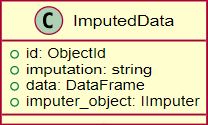
\includegraphics[width=4.5cm]{classes/model-management/16.png}}
\end{wrapfigure} 
\par
This class holds the imputed data from recent trainings.
\newline
\newline
\textbf{Attributes}
\begin{itemize}
    \item \textbf{imputation} the used imputation method
    \item \textbf{data} the imputed data
    \item \textbf{imputer\_object} the used imputer object
\end{itemize}

\subsubsection{ExtractedFeature}
\begin{wrapfigure}{l}{4.5cm}
    \raisebox{0pt}[\dimexpr\height-0.5\baselineskip\relax]{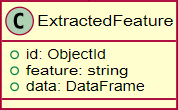
\includegraphics[width=4.5cm]{classes/model-management/17.png}}
\end{wrapfigure} 
\par
This class holds the extracted features of the data from recent trainings.
\newline
\newline
\textbf{Attributes}
\begin{itemize}
    \item \textbf{feature} the extracted feature
    \item \textbf{data} the values of the feature
\end{itemize}
